\section{Marginalization Via Message Passing}
Consider a function $f$ with factorization:
\begin{align}
\ f(x_1,x_2,x_3,x_4,x_5,x_6)=f_1(x_1,x_2,x_3)f_2(x_1,x_4,x_6)f_3(x_4)f_4(x_4, x_5)
\end{align}
Now, the marginal of function $f$ w.r.t $x_1$ is:
\begin{eqnarray}
f(x_1) 	&=&\sum_{x_2, x_3, x_4, x_5, x_6} f(x_1,x_2,x_3,x_4,x_5,x_6) \\
	&=&\left[\sum_{x_2, x_3} f_1(x_1, x_2, x_3)\right]\left[\sum_{x_4}f_3(x_4)\left(\sum_{x_6}f_2(x_1, x_4, x_6)\right)\left(\sum_{x_5}f_4(x_4, x_5)\right)\right]
%f(x_1) &=&\sum_{x_2,x_4}f_1(x_1,x_2,x_4)\,\sum_{x_3,x_6}f_2(x_3,x_4,x_6)\,\sum_{x_5,x_7}f_3(x_4,x_5,x_7)
\end{eqnarray}
Factor graph associated with above factorization is given in Figure~\ref{fig:map0}. 
\begin{figure}[htbp]
\begin{center}
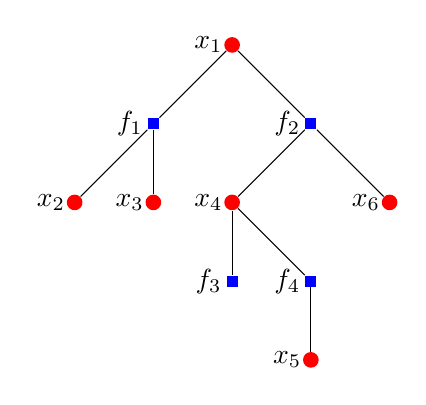
\begin{tikzpicture}[scale=1]
 \tikzstyle{cnode}=[rectangle, inner sep = 2pt, fill]
 \tikzstyle{vnode}=[circle, inner sep = 2pt, fill]
% \draw[color=red] (0,-2) node[vnode] (x2) {}; 
% \draw (-0.7, -2) node{$x_2$};
\draw [color=red](2,-2) node[vnode] (x1) {};
\draw (1.7, -2) node{$x_1$};
\draw [color=red](0,-4) node[vnode] (x2) {};
\draw (-0.3, -4) node{$x_2$};
\draw[color=red] (1,-4) node[vnode] (x3) {};
\draw (0.7, -4) node{$x_3$};
\draw[color=red] (2,-4) node[vnode] (x4) {};
\draw (1.7, -4) node{$x_4$};
\draw[color=blue] (2,-5) node[cnode] (f3) {};
\draw (1.7, -5) node{$f_3$};
\draw[color=blue] (3,-5) node[cnode] (f4) {};
\draw (2.7, -5) node{$f_4$};
\draw[color=red] (4,-4) node[vnode] (x6) {};
\draw (3.7, -4 ) node{$x_6$};
\draw[color=red] (3,-6) node[vnode] (x5) {};
\draw (2.7, -6) node{$x_5$};
\draw[color=blue] (1,-3) node[cnode] (f1) {};
\draw (0.7, -3) node{$f_1$};
\draw[color=blue] (3,-3) node[cnode] (f2) {};
\draw (2.7, -3) node{$f_2$};
\draw (x1) -- (f1);
\draw (x1) -- (f2);
\draw (f1) -- (x2);
\draw (f1) -- (x3);
\draw (f2) -- (x4);
\draw (f2) -- (x6);
\draw (x4) -- (f3);
\draw (f4) -- (x5);
\draw (x4) -- (f4);
\end{tikzpicture}
\end{center}
\caption{Factor Graph \label{fig:map0}}
\end{figure}
Here the red circles represent the variables ($x_1,x_2,\cdots,x_6$) and are called the \textit{variable-nodes}. Blue circles represent the factor ($f_1$,$f_2$,$f_3$ and $f_4$) 
and referred as the \textit{check-nodes}. In the factor graph, a variable-node is connected to a check-node iff the corresponding variable takes part in that factor.
Notice that this factor graph is a tree (i.e. there is no cycle in the graph). In the case where the factor graph is a tree the marginalization problem can be broken into smaller
tasks according to the structure of the tree. The algorithm is explained in the next paragraph

The alogorithm proceeds by sending messages along the edges of the tree. Messages are functions on $\mathcal{X}$, or equivalently, vectors of length $\left|\mathcal{X}\right|$.
The messages signify marginals of parts of the function and these parts are combined to form the marginal of the whole function. Message passing originates at the leaf nodes.
Messages are passed up the tree and as soon as a node has received messages from all its children, the incoming messages are processed and the result is passed up to the parent node.
Figure~\ref{fig:rules} explains the computation to be performed at the nodes during marginalization.

\begin{figure}[htbp]
\begin{center}
\begin{tikzpicture}[scale=1]
 \tikzstyle{cnode}=[rectangle, inner sep = 2pt, fill]
 \tikzstyle{vnode}=[circle, inner sep = 2pt, fill]
 \tikzstyle{line} = [draw, -latex']
 
 \begin{scope}
 \begin{scope}[xshift=-3cm]
    \draw[color=red] (0, 0) node[vnode] (x) {};
    \draw (0, 0.3) node{$x$};
    \draw[color=blue] (0,-1) node[cnode] (f) {};
    \draw (0, -1.3) node{$f$};
    \path [line] (f) -- node[left]{$\mu(x) = f(x)$} (x);
 \end{scope}

 \begin{scope}
  \draw (0, -0.30) node{initialization at};
  \draw (0, -0.70) node{leaf nodes};
 \end{scope}

 \begin{scope}[xshift=3cm]
    \draw[color=blue] (0, 0) node[cnode] (f) {};
    \draw (0, 0.3) node{$f$};
    \draw[color=red] (0,-1) node[vnode] (x) {};
    \draw (0, -1.3) node{$x$};
    \path [line] (x) -- node[right]{$\mu(x) = 1$} (f);  
  \end{scope}
  \end{scope}

  \begin{scope}[yshift=-3cm]
  \begin{scope}[xshift=-3cm]
 \draw[color=blue] (0, 0) node[cnode] (f) {};
 \draw (0.3, 0) node{$f$};
 \draw (0, 0.5) node{$\mu(x) = \prod_{k=1}^{K} \mu_k(x)$};
 \draw[color=red] (0,-1) node[vnode] (x) {};
 \draw (-0.3, -1) node{$x$};
 \draw[color=blue] (-1, -2) node[cnode] (f1) {};
 \draw (-1, -2.3) node{$f_1$};
 \draw[color=blue] (0, -2) node[cnode] (fk) {};
 \draw (0, -2.3) node{$f_k$};
 \draw[color=blue] (1, -2) node[cnode] (fK) {};
 \draw (1, -2.3) node{$f_K$};
 \path [line] (x) -- (f);
 \path [line] (f1) -- node[near start, left]{$\mu_1$} (x);
 \path [line] (fk) -- node[near start, left]{$\mu_k$} (x);
 \path [line] (fK) -- node[near start, right]{$\mu_K$} (x);
  \end{scope}
  
  \begin{scope}
    \draw (0, -0.80) node{variable/check};
    \draw (0, -1.20) node{node processing}; 
  \end{scope}

  \begin{scope}[xshift=3cm]
 \draw[color=red] (0, 0) node[vnode] (x) {};
 \draw (0.3, 0) node{$x$};
 \draw (0, 0.5) node{$\mu(x) = \sum_{\sim x}f(x, x_1, \cdots, x_K)\prod_{k=1}^{K} \mu_k(x)$};
 \draw[color=blue] (0,-1) node[cnode] (f) {};
 \draw (-0.3, -1) node{$f$};
 \draw[color=red] (-1, -2) node[vnode] (x1) {};
 \draw (-1, -2.3) node{$x_1$};
 \draw[color=red] (0, -2) node[vnode] (xk) {};
 \draw (0, -2.3) node{$x_k$};
 \draw[color=red] (1, -2) node[cnode] (xK) {};
 \draw (1, -2.3) node{$x_K$};
 \path [line] (f) -- (x);
 \path [line] (x1) -- node[near start, left]{$\mu_1$} (f);
 \path [line] (xk) -- node[near start, left]{$\mu_k$} (f);
 \path [line] (xK) -- node[near start, right]{$\mu_K$} (f);
  \end{scope}
  \end{scope}
  
  \begin{scope}[yshift=-7cm]
 \draw[color=blue] (0, 0) node[cnode] (f) {};
 \draw (0.5, 0) node{$f_{K + 1}$};
 \draw (0, 0.5) node{marginalization};
 \draw[color=red] (0,-1) node[vnode] (x) {};
 \draw (-0.3, -1) node{$x$};
 \draw[color=blue] (-1, -2) node[cnode] (f1) {};
 \draw (-1, -2.3) node{$f_1$};
 \draw[color=blue] (0, -2) node[cnode] (fk) {};
 \draw (0, -2.3) node{$f_k$};
 \draw[color=blue] (1, -2) node[cnode] (fK) {};
 \draw (1, -2.3) node{$f_K$};
 \draw (-1.5, -1) node{$\prod_{k=1}^{K+1} \mu_k(x)$};
 \path [line] (f) -- node[right] {$\mu_{K + 1}$} (x);
 \path [line] (f1) -- node[near start, left]{$\mu_1$} (x);
 \path [line] (fk) -- node[near start, left]{$\mu_k$} (x);
 \path [line] (fK) -- node[near start, right]{$\mu_K$} (x);
  \end{scope}
  
\end{tikzpicture}
\end{center}
\caption{Message Passing Rules \label{fig:rules}}
\end{figure}
To compute tha marginal with respect to all the variables, one can consider for each variable, a tree rooted in this variable and execute single marginal message passing algorithm 
on each rooted tree. Here all the computations can be performed simultaneously on a single tree. Start at all leaf nodes and for every edge compute the outgoing message along this
edge as soon as you have the incoming messages along all other edges that connect to a given node.
\section{Decoding Via Message Passing}
For memoryless channel without feedback, bitwise maximum a posteriori (MAP) decoding of a codeword is given by~\cite{mct}:  
\begin{align}
\hat x_i( y) &= \text{arg} \max_{x_i}p_{X_{i}|Y}(x_{i}| y) \label{eq:1}\\
\ &= \text{arg} \max_{x_i}\sum_{\sim x_i}p_{X|Y}( x| y) \label{eq:2}\\
\ &= \text{arg} \max_{x_i}\sum_{\sim x_i}p_{Y|X}( y| x)p_{X}( x) \label{eq:3}\\
\ &= \text{arg} \max_{x_i}\sum_{\sim x_i}\prod_{j}p_{Y_j|X_j}(y_j|x_j)p_{X}( x)\label{eq:4}
%\ &= \text{arg} \max_{x_i}\sum_{\sim x_i}\prod_{j}p_{Y_j/X_j}(y_j/x_j)\mathbf{1}_{x\in C}
\end{align}
The notation $\sum_{\sim x_i}$ indicates that sum is over all components of $x$, except $x_i$. 
We obtain \eqref{eq:2} from \eqref{eq:1} by total probability rule. On application of Bayes's rule,
we obtain \eqref{eq:3} from \eqref{eq:2}.
Equation \eqref{eq:2} has very high computational complexity.
For a codeword of length $n$ and rate $R$, approximate computational complexity is $\mathrm{O} (2^{nR})$. 
The computational complexity can be reduced by factorizing the sequence probability. To this end, in equation\eqref{eq:4}, 
we use the fact that the channel is memoryless, without feedback. Furthermore, since all the input codewords are equiprobable,
\begin{align}
\hat x_i(y) = \text{arg} \max_{x_i}\sum_{\sim x_i}\prod_{j}p_{Y_j|X_j}(y_j|x_j)\mathbf{1}_{\left\lbrace x\in C\right\rbrace} \label{eq:5}
\end{align} 
Where $\mathbf{1}_{\left\lbrace x\in C\right\rbrace}$ is a code membership function for the codebook $C$. Code membership function $\mathbf{1}_{\left\lbrace x\in C\right\rbrace}$
has a factorized form, and this factorization is used in efficient decoding.

\subsection{Message Passing decoder for Binary Erasure Channel}
By the standard message-passing rules the initial messages are $(\mu_j(0), \mu_j(1)) = (p_{Y_j|X_j}(y_j|0),(p_{Y_j|X_j}(y_j|1))$. In the case of binary erasure channel, the messages are
either $(1-\epsilon, 0), (\epsilon, \epsilon), \text{ or } (0, 1-\epsilon)$ corresponding to 0, ? (erasure), or 1 respectively received from channel output.
In this case we can normalize the message to (1, 0), (1, 1) and (0, 1) correspondingly. Now the message processing rules are discussed. \\
\quad \\
\textbf{Claim :} For BEC general message passing rules shown in Figure \ref{fig:rules} simplify to the following. At a variable node the outgoing message 
is an erasure if all incoming messages are erasures. Otherwise, since the channel never introduces errors, all non-erasure messages must agree and either be 0 or 1. In this case
the outgoing message is equal to this common value. At a check node the outgoing message is an erasure if anu of the incoming message is an erasure. Otherwise, if all the
incoming messages are either 0 or 1, then the outgoing message is the mod-2 sum of the incoming messages \\
\quad \\
\textbf{Proof :} If all messages entering a variable node are from the set $\left\lbrace(1, 0), (1, 1)\right\rbrace$, then the outgoing message, which is equal to the component-wise
product of the incoming messages according to the general message-passing rules, is also from this set. Further, it is equal to (1, 1) only if all incoming messages are 
of the form (1, 1) i.e, erasures. The equivalent statement is true if all incoming messages are from the set $\left\lbrace(1, 0), (1, 1)\right\rbrace$. Since channel never 
introduces errors, we only need to consider these two cases.

Next we consider the claim concerning the message-passing rule at a check node: We consider only a check node of degree 3 with two incoming messages, since check node of higher
degree can be modeled as the cascade of several check nodes, each of which has 2 inputs. Let $(\mu_1(0), \mu_1(1))$, and $(\mu_2(0), \mu_2(1))$ denote the incoming messages. By the
message processing rules the outgoing message is 
\begin{eqnarray}
 (\mu(0), \mu(1)) &=& \left( \sum_{x_1, x_2} \mathbf{1}_{\lbrace x_1 + x_2 = 0\rbrace}\mu_1(x_1)\mu_2(x_2), \sum_{x_1, x_2} \mathbf{1}_{\lbrace x_1 + x_2 = 1\rbrace}\mu_1(x_1)\mu_2(x_2)\right) \\
		  &=& \left( \mu_1(0)\mu_2(0) + \mu_1(1)\mu_2(1), \mu_1(0)\mu_2(1) + \mu_1(1)\mu_2(0)\right)
\end{eqnarray}
If $(\mu_j(0), \mu_j(1)) = (1, 1), j \in \lbrace 1, 2\rbrace$, then after normalization, $(\mu(0), \mu(1)) = (1, 1)$. Thus if any of the input is an erasure then output is an
erasure. Also if both messages are known, then by explicite check, we can see that the output corresponds to mod-2 sum. Figure~\ref{fig:message_passing} shows an example
of this decoder on (7, 4, 3) Hamming code with parity check matrix given in Equation\eqref{H_matrix}
% \documentclass[a4paper,10pt]{article}
% \usepackage[utf8]{inputenc}
% \usepackage{tikz}
% \usepackage{pgf}
% \usepackage{amsmath}
% \usepackage{textcomp}
% \usetikzlibrary{calc}
% 
% %opening
% \title{}
% \author{}
% 
% \begin{document}
% 
% \maketitle
% 
% \begin{abstract}
% 
% \end{abstract}
% 
% \section{Message Passing}
 \begin{figure}[scale=1.25]
 \centering
  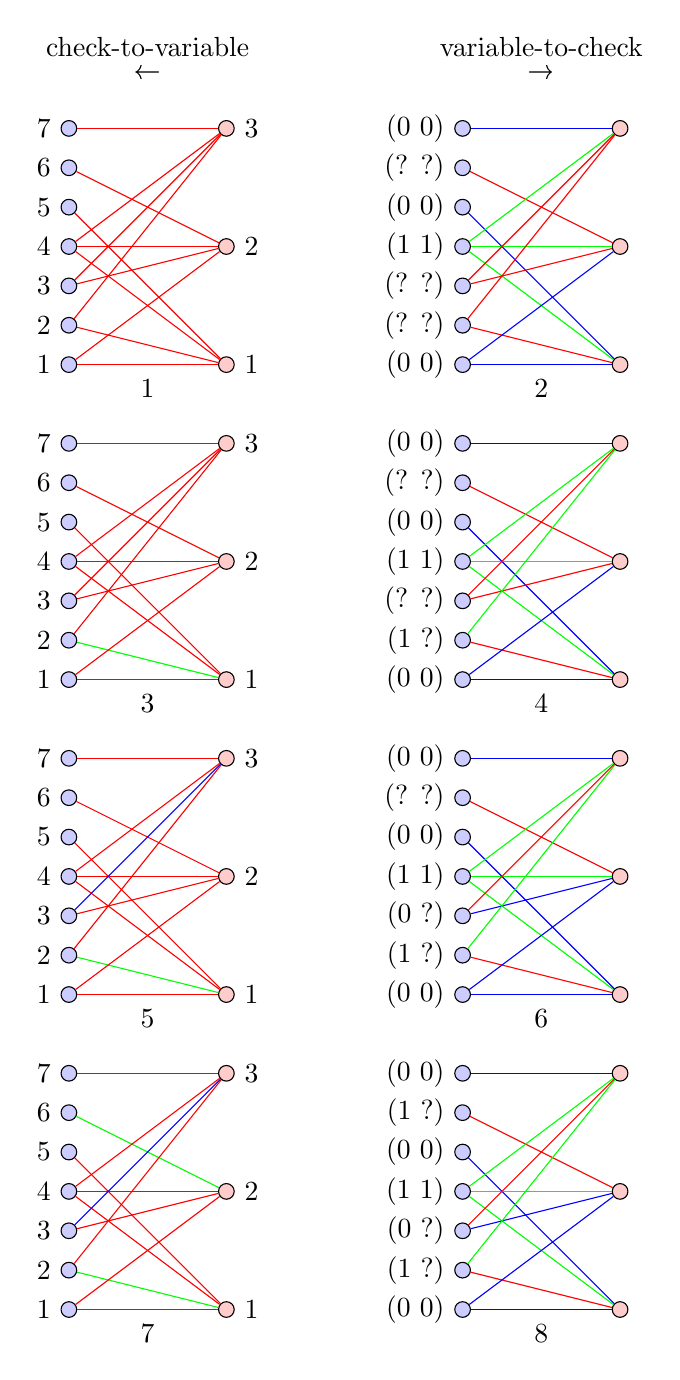
\begin{tikzpicture}
  \begin{scope}
    \begin{scope}
      \node[draw,circle,inner sep=2pt,fill=blue!20] (x7) at (0,0) [label=left:7] {};
      \node[draw,circle,inner sep=2pt,fill=blue!20] (x6) at (0,-0.5) [label=left:6] {};
      \node[draw,circle,inner sep=2pt,fill=blue!20] (x5) at (0,-1) [label=left:5] {};
      \node[draw,circle,inner sep=2pt,fill=blue!20] (x4) at (0,-1.5) [label=left:4] {};
      \node[draw,circle,inner sep=2pt,fill=blue!20] (x3) at (0,-2) [label=left:3] {};
      \node[draw,circle,inner sep=2pt,fill=blue!20] (x2) at (0,-2.5) [label=left:2] {};
      \node[draw,circle,inner sep=2pt,fill=blue!20] (x1) at (0,-3) [label=left:1] {};
      \node[draw,circle,inner sep=2pt,fill=red!20] (f3) at (2,0) [label=right:3] {};
      \node[draw,circle,inner sep=2pt,fill=red!20] (f2) at (2,-1.5) [label=right:2] {};
      \node[draw,circle,inner sep=2pt,fill=red!20] (f1) at (2,-3) [label=right:1] {};
      \draw[draw=red!100] (f1) ->  node [below = 2pt] {1} (x1);
      \draw[draw=red!100] (f1) ->  (x2);
      \draw[draw=red!100] (f1) ->  (x4);
      \draw[draw=red!100] (f1) ->  (x5);
      \draw[draw=red!100] (f2) ->  (x1);
      \draw[draw=red!100] (f2) ->  (x3);
      \draw[draw=red!100] (f2) ->  (x4);
      \draw[draw=red!100] (f2) ->  (x6);
      \draw[draw=red!100] (f3) ->  (x2);
      \draw[draw=red!100] (f3) ->  (x3);
      \draw[draw=red!100] (f3) ->  (x4);
      \draw[draw=red!100] (f3) -> node [above = 0.5cm] (larrow) {\textleftarrow} (x7);
      \node[above of=larrow, node distance=10pt] {check-to-variable};
    \end{scope}
    \begin{scope}[yshift=-4cm]
      \node[draw,circle,inner sep=2pt,fill=blue!20] (x7) at (0,0) [label=left:7] {};
      \node[draw,circle,inner sep=2pt,fill=blue!20] (x6) at (0,-0.5) [label=left:6] {};
      \node[draw,circle,inner sep=2pt,fill=blue!20] (x5) at (0,-1) [label=left:5] {};
      \node[draw,circle,inner sep=2pt,fill=blue!20] (x4) at (0,-1.5) [label=left:4] {};
      \node[draw,circle,inner sep=2pt,fill=blue!20] (x3) at (0,-2) [label=left:3] {};
      \node[draw,circle,inner sep=2pt,fill=blue!20] (x2) at (0,-2.5) [label=left:2] {};
      \node[draw,circle,inner sep=2pt,fill=blue!20] (x1) at (0,-3) [label=left:1] {};
      \node[draw,circle,inner sep=2pt,fill=red!20] (f3) at (2,0) [label=right:3] {};
      \node[draw,circle,inner sep=2pt,fill=red!20] (f2) at (2,-1.5) [label=right:2] {};
      \node[draw,circle,inner sep=2pt,fill=red!20] (f1) at (2,-3) [label=right:1] {};
      \draw[draw=red!100] (f1) ->  node [below = 2pt] {3} (x1);
      \draw[draw=green!100] (f1) ->  (x2);
      \draw[draw=red!100] (f1) ->  (x4);
      \draw[draw=red!100] (f1) ->  (x5);
      \draw[draw=red!100] (f2) ->  (x1);
      \draw[draw=red!100] (f2) ->  (x3);
      \draw[draw=red!100] (f2) ->  (x4);
      \draw[draw=red!100] (f2) ->  (x6);
      \draw[draw=red!100] (f3) ->  (x2);
      \draw[draw=red!100] (f3) ->  (x3);
      \draw[draw=red!100] (f3) ->  (x4);
      \draw[draw=red!100] (f3) ->  (x7);
    \end{scope}
    \begin{scope}[yshift=-8cm]
      \node[draw,circle,inner sep=2pt,fill=blue!20] (x7) at (0,0) [label=left:7] {};
      \node[draw,circle,inner sep=2pt,fill=blue!20] (x6) at (0,-0.5) [label=left:6] {};
      \node[draw,circle,inner sep=2pt,fill=blue!20] (x5) at (0,-1) [label=left:5] {};
      \node[draw,circle,inner sep=2pt,fill=blue!20] (x4) at (0,-1.5) [label=left:4] {};
      \node[draw,circle,inner sep=2pt,fill=blue!20] (x3) at (0,-2) [label=left:3] {};
      \node[draw,circle,inner sep=2pt,fill=blue!20] (x2) at (0,-2.5) [label=left:2] {};
      \node[draw,circle,inner sep=2pt,fill=blue!20] (x1) at (0,-3) [label=left:1] {};
      \node[draw,circle,inner sep=2pt,fill=red!20] (f3) at (2,0) [label=right:3] {};
      \node[draw,circle,inner sep=2pt,fill=red!20] (f2) at (2,-1.5) [label=right:2] {};
      \node[draw,circle,inner sep=2pt,fill=red!20] (f1) at (2,-3) [label=right:1] {};
      \draw[draw=red!100] (f1) ->  node [below = 2pt] {5} (x1);
      \draw[draw=green!100] (f1) ->  (x2);
      \draw[draw=red!100] (f1) ->  (x4);
      \draw[draw=red!100] (f1) ->  (x5);
      \draw[draw=red!100] (f2) ->  (x1);
      \draw[draw=red!100] (f2) ->  (x3);
      \draw[draw=red!100] (f2) ->  (x4);
      \draw[draw=red!100] (f2) ->  (x6);
      \draw[draw=red!100] (f3) ->  (x2);
      \draw[draw=blue!100] (f3) ->  (x3);
      \draw[draw=red!100] (f3) ->  (x4);
      \draw[draw=red!100] (f3) ->  (x7);
    \end{scope}
    \begin{scope}[yshift=-12cm]
      \node[draw,circle,inner sep=2pt,fill=blue!20] (x7) at (0,0) [label=left:7] {};
      \node[draw,circle,inner sep=2pt,fill=blue!20] (x6) at (0,-0.5) [label=left:6] {};
      \node[draw,circle,inner sep=2pt,fill=blue!20] (x5) at (0,-1) [label=left:5] {};
      \node[draw,circle,inner sep=2pt,fill=blue!20] (x4) at (0,-1.5) [label=left:4] {};
      \node[draw,circle,inner sep=2pt,fill=blue!20] (x3) at (0,-2) [label=left:3] {};
      \node[draw,circle,inner sep=2pt,fill=blue!20] (x2) at (0,-2.5) [label=left:2] {};
      \node[draw,circle,inner sep=2pt,fill=blue!20] (x1) at (0,-3) [label=left:1] {};
      \node[draw,circle,inner sep=2pt,fill=red!20] (f3) at (2,0) [label=right:3] {};
      \node[draw,circle,inner sep=2pt,fill=red!20] (f2) at (2,-1.5) [label=right:2] {};
      \node[draw,circle,inner sep=2pt,fill=red!20] (f1) at (2,-3) [label=right:1] {};
      \draw[draw=red!100] (f1) ->  node [below = 2pt] {7} (x1);
      \draw[draw=green!100] (f1) ->  (x2);
      \draw[draw=red!100] (f1) ->  (x4);
      \draw[draw=red!100] (f1) ->  (x5);
      \draw[draw=red!100] (f2) ->  (x1);
      \draw[draw=red!100] (f2) ->  (x3);
      \draw[draw=red!100] (f2) ->  (x4);
      \draw[draw=green!100] (f2) ->  (x6);
      \draw[draw=red!100] (f3) ->  (x2);
      \draw[draw=blue!100] (f3) ->  (x3);
      \draw[draw=red!100] (f3) ->  (x4);
      \draw[draw=red!100] (f3) ->  (x7);
    \end{scope}
  \end{scope}
%=========================================================================================
  \begin{scope}[xshift=5cm]
    \begin{scope}
      \node[draw,circle,inner sep=2pt,fill=blue!20] (x7) at (0,0) [label=left:(0 0)] {};
      \node[draw,circle,inner sep=2pt,fill=blue!20] (x6) at (0,-0.5) [label=left:(? ?)] {};
      \node[draw,circle,inner sep=2pt,fill=blue!20] (x5) at (0,-1) [label=left:(0 0)] {};
      \node[draw,circle,inner sep=2pt,fill=blue!20] (x4) at (0,-1.5) [label=left:(1 1)] {};
      \node[draw,circle,inner sep=2pt,fill=blue!20] (x3) at (0,-2) [label=left:(? ?)] {};
      \node[draw,circle,inner sep=2pt,fill=blue!20] (x2) at (0,-2.5) [label=left:(? ?)] {};
      \node[draw,circle,inner sep=2pt,fill=blue!20] (x1) at (0,-3) [label=left:(0 0)] {};
      \node[draw,circle,inner sep=2pt,fill=red!20] (f3) at (2,0) {};
      \node[draw,circle,inner sep=2pt,fill=red!20] (f2) at (2,-1.5) {};
      \node[draw,circle,inner sep=2pt,fill=red!20] (f1) at (2,-3) {};
      \draw[draw=blue!100] (f1) ->  node [below = 2pt] {2} (x1);
      \draw[draw=red!100] (f1) ->  (x2);
      \draw[draw=green!100] (f1) ->  (x4);
      \draw[draw=blue!100] (f1) ->  (x5);
      \draw[draw=blue!100] (f2) ->  (x1);
      \draw[draw=red!100] (f2) ->  (x3);
      \draw[draw=green!100] (f2) ->  (x4);
      \draw[draw=red!100] (f2) ->  (x6);
      \draw[draw=red!100] (f3) ->  (x2);
      \draw[draw=red!100] (f3) ->  (x3);
      \draw[draw=green!100] (f3) ->  (x4);
      \draw[draw=blue!100] (f3) -> node [above = 0.5cm] (rarrow) {\textrightarrow} (x7);
      \node[above of=rarrow, node distance=10pt] {variable-to-check};
    \end{scope}
    \begin{scope}[yshift=-4cm]
      \node[draw,circle,inner sep=2pt,fill=blue!20] (x7) at (0,0) [label=left:(0 0)] {};
      \node[draw,circle,inner sep=2pt,fill=blue!20] (x6) at (0,-0.5) [label=left:(? ?)] {};
      \node[draw,circle,inner sep=2pt,fill=blue!20] (x5) at (0,-1) [label=left:(0 0)] {};
      \node[draw,circle,inner sep=2pt,fill=blue!20] (x4) at (0,-1.5) [label=left:(1 1)] {};
      \node[draw,circle,inner sep=2pt,fill=blue!20] (x3) at (0,-2) [label=left:(? ?)] {};
      \node[draw,circle,inner sep=2pt,fill=blue!20] (x2) at (0,-2.5) [label=left:(1 ?)] {};
      \node[draw,circle,inner sep=2pt,fill=blue!20] (x1) at (0,-3) [label=left:(0 0)] {};
      \node[draw,circle,inner sep=2pt,fill=red!20] (f3) at (2,0) {};
      \node[draw,circle,inner sep=2pt,fill=red!20] (f2) at (2,-1.5) {};
      \node[draw,circle,inner sep=2pt,fill=red!20] (f1) at (2,-3) {};
      \draw[draw=blue!100] (f1) ->  node [below = 2pt] {4} (x1);
      \draw[draw=red!100] (f1) ->  (x2);
      \draw[draw=green!100] (f1) ->  (x4);
      \draw[draw=blue!100] (f1) ->  (x5);
      \draw[draw=blue!100] (f2) ->  (x1);
      \draw[draw=red!100] (f2) ->  (x3);
      \draw[draw=green!100] (f2) ->  (x4);
      \draw[draw=red!100] (f2) ->  (x6);
      \draw[draw=green!100] (f3) ->  (x2);
      \draw[draw=red!100] (f3) ->  (x3);
      \draw[draw=green!100] (f3) ->  (x4);
      \draw[draw=blue!100] (f3) ->  (x7);
    \end{scope}
    \begin{scope}[yshift=-8cm]
      \node[draw,circle,inner sep=2pt,fill=blue!20] (x7) at (0,0) [label=left:(0 0)] {};
      \node[draw,circle,inner sep=2pt,fill=blue!20] (x6) at (0,-0.5) [label=left:(? ?)] {};
      \node[draw,circle,inner sep=2pt,fill=blue!20] (x5) at (0,-1) [label=left:(0 0)] {};
      \node[draw,circle,inner sep=2pt,fill=blue!20] (x4) at (0,-1.5) [label=left:(1 1)] {};
      \node[draw,circle,inner sep=2pt,fill=blue!20] (x3) at (0,-2) [label=left:(0 ?)] {};
      \node[draw,circle,inner sep=2pt,fill=blue!20] (x2) at (0,-2.5) [label=left:(1 ?)] {};
      \node[draw,circle,inner sep=2pt,fill=blue!20] (x1) at (0,-3) [label=left:(0 0)] {};
      \node[draw,circle,inner sep=2pt,fill=red!20] (f3) at (2,0) {};
      \node[draw,circle,inner sep=2pt,fill=red!20] (f2) at (2,-1.5) {};
      \node[draw,circle,inner sep=2pt,fill=red!20] (f1) at (2,-3) {};
      \draw[draw=blue!100] (f1) ->  node [below = 2pt] {6} (x1);
      \draw[draw=red!100] (f1) ->  (x2);
      \draw[draw=green!100] (f1) ->  (x4);
      \draw[draw=blue!100] (f1) ->  (x5);
      \draw[draw=blue!100] (f2) ->  (x1);
      \draw[draw=blue!100] (f2) ->  (x3);
      \draw[draw=green!100] (f2) ->  (x4);
      \draw[draw=red!100] (f2) ->  (x6);
      \draw[draw=green!100] (f3) ->  (x2);
      \draw[draw=red!100] (f3) ->  (x3);
      \draw[draw=green!100] (f3) ->  (x4);
      \draw[draw=blue!100] (f3) ->  (x7);
    \end{scope}
    \begin{scope}[yshift=-12cm]
      \node[draw,circle,inner sep=2pt,fill=blue!20] (x7) at (0,0) [label=left:(0 0)] {};
      \node[draw,circle,inner sep=2pt,fill=blue!20] (x6) at (0,-0.5) [label=left:(1 ?)] {};
      \node[draw,circle,inner sep=2pt,fill=blue!20] (x5) at (0,-1) [label=left:(0 0)] {};
      \node[draw,circle,inner sep=2pt,fill=blue!20] (x4) at (0,-1.5) [label=left:(1 1)] {};
      \node[draw,circle,inner sep=2pt,fill=blue!20] (x3) at (0,-2) [label=left:(0 ?)] {};
      \node[draw,circle,inner sep=2pt,fill=blue!20] (x2) at (0,-2.5) [label=left:(1 ?)] {};
      \node[draw,circle,inner sep=2pt,fill=blue!20] (x1) at (0,-3) [label=left:(0 0)] {};
      \node[draw,circle,inner sep=2pt,fill=red!20] (f3) at (2,0) {};
      \node[draw,circle,inner sep=2pt,fill=red!20] (f2) at (2,-1.5) {};
      \node[draw,circle,inner sep=2pt,fill=red!20] (f1) at (2,-3) {};
      \draw[draw=blue!100] (f1) ->  node [below = 2pt] {8} (x1);
      \draw[draw=red!100] (f1) ->  (x2);
      \draw[draw=green!100] (f1) ->  (x4);
      \draw[draw=blue!100] (f1) ->  (x5);
      \draw[draw=blue!100] (f2) ->  (x1);
      \draw[draw=blue!100] (f2) ->  (x3);
      \draw[draw=green!100] (f2) ->  (x4);
      \draw[draw=red!100] (f2) ->  (x6);
      \draw[draw=green!100] (f3) ->  (x2);
      \draw[draw=red!100] (f3) ->  (x3);
      \draw[draw=green!100] (f3) ->  (x4);
      \draw[draw=blue!100] (f3) ->  (x7);
    \end{scope}
  \end{scope}
  \end{tikzpicture}
\caption{Message-passing decoding of the [7, 4, 3] Hamming code with the received code word y = (0, ?, ?, 1, 0, ?, 0).
The left column is represents message passing from check to variable nodes. Right column represents message passing
from variable to check nodes. Red links represents erasure messages, blue links represents messages 1 (corresponds to codebit 0)
and green links represents message -1 (corresponds to codebit 1). The labels on the variable nodes in the right column represents
the pair (estimated bit, received bit)}
\label{fig:message_passing}
\end{figure}
% \end{document}
\subsection{Message Passing Decoder for Binary Input AWGN Channel}
 \begin{figure}[scale=1.25]
 \centering
  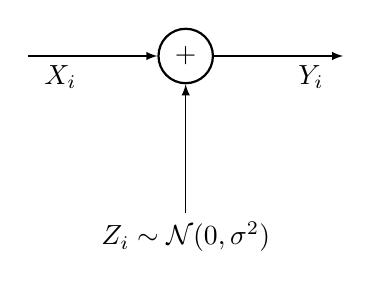
\begin{tikzpicture}
  \draw (0, 0) node[circle, thick, draw] (f) {$+$};
  \path [draw, -latex] (-2, 0) -- node[near start, below]{$X_i$}(f) ;
  \path [draw, -latex] (f) -- node[near end, below]{$Y_i$}(2, 0) ;
  \path [draw, -latex] (0, -2) -- (f);
  \draw (0, -2.3) node{$Z_i \sim \mathcal{N}(0, \sigma^2)$};
   \end{tikzpicture}
\caption{AWGN Channel}
\label{fig:awgn_channel}
\end{figure}


Given in Figure~\ref{fig:awgn_channel} is a mathematical model of AWGN channel.
We think that the channel input $x_i \in \lbrace -1, +1\rbrace$.
Here again a message can be thought of as a real-valued vector of length 2, $(\mu(-1), \mu(1))$. We initialize the message passing iterations by sending from 
$i^{th}$ variable node the vector $(p_{Y_i|X_i}(y_i|-1), p_{Y_i|X_i}(y_i|1))$. In case of binary input channels, it suffices to send the log-likelihood ratios.
 \begin{equation*}
 l = \log \left(\dfrac{\mu(-1)}{\mu(1)}\right)
 \end{equation*}
On using log-likelihood ratios, the message passing rules simplipy to the following. At variable node, simply add the incoming messages and at a check node of degree $J + 1$,
use the following computation.
\begin{equation}
 l = 2 \arctanh \left( \prod_{j=1}^J \tanh \left(l_j/2\right)\right) 
\end{equation}
In the case of Binary Input AWGN Channel, we can initialize the message passing iterations by sending 
\begin{eqnarray}
 l_i &=& \log \left(\dfrac{\mu(-1)}{\mu(1)}\right) \\
     &=& \log \left(\dfrac{p_{Y_i|X_i}(y_i|-1)}{p_{Y_i|X_i}(y_i|1)}\right) \\
     &=& \dfrac{-2y_i}{\sigma^2}
\end{eqnarray}
from variable nodes to the check nodes. Further computations are carried out as expained above.
One iteration consists of message passing from variable nodes to check nodes, computations at the check nodes and 
message passing from check nodes to variable nodes. After one such iteration, we find the probability ratios by the marginalization
step shown in the Figure~\ref{fig:rules}. Based on the probability ratios, we estimate the codeword, by the following rule. If the probability ratio is greater than 0, we decode that bit
in favor of -1 and else in favor of 1. We check if the estimated codeword is an actual codeword by parity checks. If the estimated codeword is an actual codeword, we stop, else
we continue with the next round of message passing iterations.